\PassOptionsToPackage{table}{xcolor}
\documentclass[pdf]{beamer}
\mode<presentation>{\usetheme{Dresden}}
\usepackage{lmodern}
\usepackage[normalem]{ulem}
\usepackage{amsmath,textcomp,amssymb,geometry,graphicx,listings,array,color,amsthm}

\usepackage[noend]{algpseudocode}

\usepackage{tikz}
\usepackage{multicol}
\usetikzlibrary{shapes,snakes}
\usetikzlibrary{positioning}
\usetikzlibrary{arrows}
\usetikzlibrary{fit}
\usetikzlibrary{math}

%% For on-slide alerting of nodes
\tikzstyle{alert} = [text=black, fill=blue!20, draw=black]
\setbeamercolor{alerted text}{fg=blue}
\tikzset{alerton/.code args={<#1>}{%
  \only<#1>{\pgfkeysalso{alert}} % \pgfkeysalso doesn't change the path
}}

%% utils for removing uninteresting sections from the navbar
%% https://tex.stackexchange.com/questions/317774/hide-section-from-sidebar
\makeatletter
\let\beamer@writeslidentry@miniframeson=\beamer@writeslidentry%
\def\beamer@writeslidentry@miniframesoff{%
  \expandafter\beamer@ifempty\expandafter{\beamer@framestartpage}{}% does not happen normally
  {%else
    % removed \addtocontents commands
    \clearpage\beamer@notesactions%
  }
}
\newcommand*{\miniframeson}{\let\beamer@writeslidentry=\beamer@writeslidentry@miniframeson}
\newcommand*{\miniframesoff}{\let\beamer@writeslidentry=\beamer@writeslidentry@miniframesoff}
\makeatother

%% preamble
\title{Prisoner's Dilemma}
\subtitle{Theme and Variations}
\author{A.C.}
\date{\today}

\AtBeginSection[]
{
  \miniframesoff
  \begin{frame}{Outline}
    \tableofcontents[currentsection,hideothersubsections]
  \end{frame}
  \miniframeson
}

\definecolor{darkred}{rgb}{0.7,0,0}
\definecolor{darkgreen}{rgb}{0,0.5,0}
\definecolor{darkblue}{rgb}{0,0,0.5}
\definecolor{darkpurple}{rgb}{0.4, 0.0, 0.4}

%% Code font settings
\lstset{
  showstringspaces=false,
  basicstyle=\scriptsize\ttfamily,
  commentstyle=\color{darkred},
  stringstyle=\color{darkgreen},
  keywordstyle=\bfseries\color{darkpurple},
}

%%%%%%%%%%%%%%%%%%%%%%%%%%
% Start of Actual slides %
%%%%%%%%%%%%%%%%%%%%%%%%%%
\begin{document}
\begin{frame}
  \titlepage
\end{frame}

\section{The Prisoner's Dilemma}
\subsection{Single Round}
\begin{frame}{Nash Equilibrium}
  We say that players in a non-cooperative game are in a \textbf{Nash Equilibrium}
  if neither can improve their score by adopting a new strategy.
  \begin{itemize}
  \pause\item Players \emph{can} communicate. Their strategies are assumed transparent
    to each other.
  \pause\item Players \emph{cannot} cooperate. It's still a Nash Equilibrium if both
    players changing strategy together yields improvement.
  \end{itemize}
\end{frame}

\begin{frame}{Prisoner's Dilemma}
  % TODO: insert a 2x2 showing the Axelrod reward/punish matrix

  % Notes:
  % - Stage game
  % - Optimal play: Defect
  % - Nash Equilibrium
  % - Opponent-independent
\end{frame}

\begin{frame}{Homo Economicus}
  \begin{center}
    
\includegraphics[scale=0.20]{skinner_homo_economicus.jpg}
  \end{center}
\end{frame}

\subsection{Fixed, Finite Rounds}

\begin{frame}{Iterated Prisoner's Dilemma}

  What happens if we play several rounds of prisoner's dilemma? A tension
  between developing good will (cooperating) and spending it (defecting)?

  Simple rules:
  \begin{itemize}
  \item $N$ rounds of play.
  \item Same reward-space in every round.
  \item Final score is sum of individual rounds.
  \item Every player has perfect recall.
  \end{itemize}
\end{frame}

\begin{frame}{Rational Play}
  \begin{itemize}
  \item Final round reduces to plain PD;
    \begin{itemize}
      \item D-D
    \end{itemize}
  \pause\item Penultimate round reduces to plain PD, followed by D-D.
    \begin{itemize}
      \item D-D, D-D
    \end{itemize}
  \pause\item round before that reduces to plain PD, followed by D-D, D-D.
    \begin{itemize}
      \item D-D, D-D, D-D
    \end{itemize}
  \pause\item $\ldots$
  \pause\item $\ldots$
  \pause\item D-D,D-D,D-D,$\ldots$,D-D
\end{itemize}
\end{frame}

\begin{frame}{Greater Fools}
  \begin{itemize}
  \item Iterated PD still yields universal defection under optimal, rational play.
  \pause\item Irrational partners could cooperate.
  \begin{itemize}
    \item We might want to (sometimes) cooperate as well, depending on partner.
    \end{itemize}
  \end{itemize}
\end{frame}


\subsection{Infinite Rounds}
\begin{frame}{Infinite Round Prisoner's Dilemma}
  What happens if we play forever?

  \begin{itemize}
  \item $\infty$ rounds of play.
  \item Same reward-space in every round.
  \item Every player has perfect recall.
  \item Final score is the \emph{discounted} sum of individual rounds.
    \begin{itemize}
    \item $s = \sum \gamma^n s_n$ for a fixed discount factor $\gamma \in [0, 1)$
    \pause\item Encodes a bird-in-the-hand sensibility, or stochastic early stopping
    \pause\item Also, it makes the sum converge.
    \end{itemize}
  \end{itemize}
\end{frame}

\begin{frame}{Defect Always}
  \begin{itemize}
    \item Let player A plan to always defect.
    \pause\item Player B obviously has no incentive to cooperate, will also plan to defect.
    \pause\item By symmetry, A also has no incentive to cooperate.
  \end{itemize}\pause
 
  Defect-always is still \emph{an} equilibrium.
\end{frame}

\begin{frame}{Grim Trigger}
  \begin{itemize}
    \item Let players A and B plan to cooperate until defect.
    \begin{itemize}
      \item After first defection, each player plans to revert to defect-always.
    \end{itemize}
    \pause\item First defector scores a C-D bonus, but all future rounds will be D-D.
    \pause\item If $\gamma$ is large enough, nobody will ever want to defect.
    \begin{itemize}
      \item Can apply OSDP if more rigor is desired.
    \end{itemize}
  \end{itemize}

  \pause Grim Trigger is an always-cooperating equilibrium.
\end{frame}

\begin{frame}{Credibility}
  Cooperation in $\infty$-PD possible only with credible retaliation.

  \pause
  \begin{itemize}
  \item Strategies are immutable.
  \item Strategies are published.
  \end{itemize}

  \pause
  How realistic is that, anyways?
\end{frame}

\begin{frame}{Credibility II: Roko's Basilisk}
  \begin{center}
    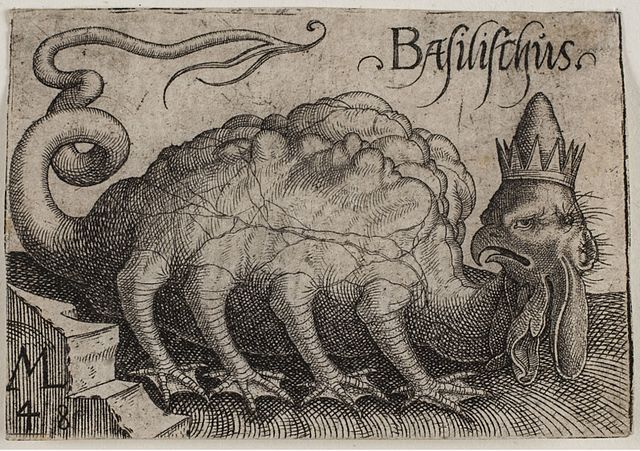
\includegraphics[scale=0.25]{basilisk.jpg}
  \end{center}
\end{frame}

\begin{frame}{Credibility III: Declaratory Strategy}
  \begin{center}
    
\includegraphics[scale=0.2]{npr_title_page_2022.png}
  \end{center}
\end{frame}

\section{Axelrod's Tournament}
\subsection{Axelrod's Tournament}
\begin{frame}{Tournament Format}
\end{frame}
\begin{frame}{Tit-for-Tat}
\end{frame}
\begin{frame}{Grim Trigger}
\end{frame}
\begin{frame}{Win-Stay, Lose-Switch}
\end{frame}
\begin{frame}{Tournament Results}
\end{frame}
\begin{frame}{Objective Re-alignment}
\end{frame}
\begin{frame}{Founder Effects}
\end{frame}
\begin{frame}{The Red Queen}
\end{frame}

\subsection{Noisy PD}
\begin{frame}{Mixed Signals}
  Problem variant: Cooperate/Defect decision is randomly flipped with some probability $p$.\newline

  What happens?
\end{frame}
\begin{frame}{TFT}
  C-C\pause, C-C\pause, C-C\pause, \textcolor{darkred}{D}-C\pause, C-D\pause,D-C\pause,$\ldots$\pause

  \begin{itemize}
  \item Cooperate-then-defect chain continues until an error or error(s) puts us into C-C again.
    \pause
  \item Harder to fall out of the non-cooperation loop than into it.
  \end{itemize}
\end{frame}

\begin{frame}{TF2T}
  Simple robustification strategy: retaliate only on two defects:\pause
  
  C-C\pause, C-C\pause, C-C\pause, \textcolor{darkred}{D}-C\pause, C-C\pause, C-C\pause,$\ldots$

  \begin{itemize}
  \item Very difficult to fall into accidental conflict.
    \pause
  \item No harder to fall out of it.
    \pause
  \item Can be exploited by ``predatory'' strategies.
  \end{itemize}
  
\end{frame}

\section{Single-Round Cooperation}
\begin{frame}{Super-Rationality}
\end{frame}

\begin{frame}{Mutual Interest}
\end{frame}

\end{document}
